\documentclass[aps,prc,reprint,amsmath,nofootinbib]{revtex4-1}

\usepackage[utf8]{inputenc}
\usepackage{amsmath}
\usepackage{amssymb}
\usepackage{multirow}

\usepackage{color}
\definecolor{theblue}{RGB}{0,50,230}

\usepackage{hyperref}
\hypersetup{
  colorlinks=true,
  linkcolor=theblue,
  citecolor=theblue,
  urlcolor=theblue
}

\usepackage{tikz}

\usepackage{graphicx}
\graphicspath{{../plots/}}

\newcommand{\trento}{T\raisebox{-0.5ex}{R}ENTo}
\newcommand{\avg}[1]{\langle #1 \rangle}
\newcommand{\nch}{N_\text{ch}}
\newcommand{\npart}{N_\text{part}}
\newcommand{\sqrts}{\sqrt{s_{NN}}}
\newcommand{\T}{\tilde{T}}
\newcommand{\vnk}[2]{v_#1\{#2\}}
\newcommand{\paddedhline}{\noalign{\smallskip}\hline\noalign{\smallskip}}
\newcommand{\order}[1]{$\mathcal O(10^{#1})$}
\newcommand{\note}{\textcolor{theblue}{[?]}}

% Convenient figure macro.  Usage:
%
%   \fig[placement specifier = t]{filename}{caption}
%
% This creates a figure environment, includes the given filename as graphics,
% puts the given caption below the graphics, and labels it 'fig:filename'.
% The optional placement specifier defaults to 't' and is passed directly to
% the figure environment.
% Use \fig* to make a figure* environment, i.e. a wide figure.
\usepackage{xparse}
\NewDocumentCommand\fig{sO{t}mm}{
  \begin{figure\IfBooleanT{#1}{*}}[#2]
    \includegraphics{#3}
    \caption{\label{fig:#3}#4}
  \end{figure\IfBooleanT{#1}{*}}
}


\begin{document}

\title{
  Estimating initial state and quark-gluon plasma medium properties\\
  using a hydrodynamic model with nucleon substructure\\calibrated to p-Pb and Pb-Pb collisions at $\sqrts=5.02$~TeV
}

\author{J.\ Scott Moreland}
\author{Jonah E.\ Bernhard}
\author{Steffen A.\ Bass}
\affiliation{Department of Physics, Duke University, Durham, NC 27708-0305}

\date{\today}

\begin{abstract}
  We posit a unified hydrodynamic description of ultrarelativistic $p$-Pb and Pb-Pb nuclear collisions at $\sqrts=5.02$~TeV and evaluate the likelihood of our assertion using Bayesian inference.
  Specifically, we model the dynamics of both collision systems using QGP initial conditions with parametric nucleon substructure, a pre-equilibrium free-streaming stage, event-by-event viscous hydrodynamics, and a microscopic hadronic afterburner.
  Free parameters of the model which describe the initial state and QGP medium are then simultaneously calibrated to fit charged particle yields, mean $p_T$ and flow cumulants of both systems.
  We argue that the global agreement of the calibrated model with available experimental data strongly supports the existence of hydrodynamic flow in small collision systems at ultrarelativistic energies, and that this flow necessarily develops at length scales smaller than a proton.
  Finally, we present posterior distributions on our model's initial state and QGP medium parameters, including new constraints on the shape and structure of the proton.
\end{abstract}

\maketitle


\section{Introduction}
  Ultrarelativistic collisions of light and light-heavy \mbox{(e.g.\ $p$-$p$ and $p$-Pb)} ion pairs produce long-range multiparticle correlations which are striking similar to those observed in heavy-ion collisions \note, where the observed collectivity is commonly attributed to hydrodynamic flow \note.
  This observation suggests that hydrodynamic behavior could be manifest in small droplets of quark-gluon-plasma (QGP), and that flow might develop at length scales smaller than a proton.

 Lorem ipsum dolor sit amet, consectetur adipiscing elit. In tincidunt elit a libero luctus, ut pharetra sem accumsan. Nullam eros dui, egestas ut arcu et, commodo suscipit purus. Quisque dapibus tincidunt nulla at vehicula. Nulla ut libero sapien. Suspendisse ac consectetur metus. Interdum et malesuada fames ac ante ipsum primis in faucibus. Nunc facilisis volutpat suscipit. Pellentesque nec est orci. Donec id pharetra enim.

Aliquam porttitor massa risus, hendrerit dignissim purus placerat vel. Suspendisse dui ante, porttitor pretium lorem et, placerat posuere mi. Donec lacinia nisl leo, ac luctus libero tincidunt non. Donec pretium ultricies felis vitae tempus. Duis pulvinar nisi justo, sit amet finibus orci volutpat non. Proin fermentum a magna id rhoncus. Vestibulum posuere, ipsum vel dignissim laoreet, arcu nibh venenatis neque, et aliquet dui dui a ipsum. Praesent sagittis condimentum neque, sed aliquam odio volutpat nec. Aenean consequat ante eget mauris lacinia, sed ultrices est dapibus. Morbi fermentum malesuada turpis, ac placerat est bibendum tincidunt. Nullam leo ipsum, sodales sit amet viverra non, iaculis vel nisl. Vestibulum purus ipsum, egestas ut bibendum sed, congue quis purus. Curabitur iaculis tortor nisl, nec venenatis tortor placerat a. Fusce feugiat nisl vitae porta porta. Praesent non arcu leo. Sed gravida eget neque in auctor.

Sed ac ullamcorper ipsum. Sed quis eleifend mauris. Phasellus quis massa neque. Proin nec lectus quis ante aliquam tincidunt ut sit amet eros. Nullam et odio eu elit aliquam molestie quis ut arcu. Aliquam gravida enim non tortor bibendum, at semper tellus egestas. In libero lectus, convallis in suscipit nec, bibendum eu felis. Vestibulum ante ipsum primis in faucibus orci luctus et ultrices posuere cubilia Curae; Vivamus quis lectus neque. Sed ac placerat justo. Nullam ultricies vulputate ligula, vel porta mauris scelerisque et. Sed hendrerit blandit semper. Sed vel bibendum elit, eu posuere elit. Phasellus nunc massa, tincidunt ac tempus quis, blandit quis erat. 

\section{Nuclear collision model}

 Lorem ipsum dolor sit amet, consectetur adipiscing elit. In tincidunt elit a libero luctus, ut pharetra sem accumsan. Nullam eros dui, egestas ut arcu et, commodo suscipit purus. Quisque dapibus tincidunt nulla at vehicula. Nulla ut libero sapien. Suspendisse ac consectetur metus. Interdum et malesuada fames ac ante ipsum primis in faucibus. Nunc facilisis volutpat suscipit. Pellentesque nec est orci. Donec id pharetra enim.

\subsection{Initial conditions}

Aliquam porttitor massa risus, hendrerit dignissim purus placerat vel. Suspendisse dui ante, porttitor pretium lorem et, placerat posuere mi. Donec lacinia nisl leo, ac luctus libero tincidunt non. Donec pretium ultricies felis vitae tempus. Duis pulvinar nisi justo, sit amet finibus orci volutpat non. Proin fermentum a magna id rhoncus. Vestibulum posuere, ipsum vel dignissim laoreet, arcu nibh venenatis neque, et aliquet dui dui a ipsum. Praesent sagittis condimentum neque, sed aliquam odio volutpat nec. Aenean consequat ante eget mauris lacinia, sed ultrices est dapibus. Morbi fermentum malesuada turpis, ac placerat est bibendum tincidunt. Nullam leo ipsum, sodales sit amet viverra non, iaculis vel nisl. Vestibulum purus ipsum, egestas ut bibendum sed, congue quis purus. Curabitur iaculis tortor nisl, nec venenatis tortor placerat a. Fusce feugiat nisl vitae porta porta. Praesent non arcu leo. Sed gravida eget neque in auctor.

\subsection{Pre-equilibrium dynamics}

Sed ac ullamcorper ipsum. Sed quis eleifend mauris. Phasellus quis massa neque. Proin nec lectus quis ante aliquam tincidunt ut sit amet eros. Nullam et odio eu elit aliquam molestie quis ut arcu. Aliquam gravida enim non tortor bibendum, at semper tellus egestas. In libero lectus, convallis in suscipit nec, bibendum eu felis. Vestibulum ante ipsum primis in faucibus orci luctus et ultrices posuere cubilia Curae; Vivamus quis lectus neque. Sed ac placerat justo. Nullam ultricies vulputate ligula, vel porta mauris scelerisque et. Sed hendrerit blandit semper. Sed vel bibendum elit, eu posuere elit. Phasellus nunc massa, tincidunt ac tempus quis, blandit quis erat. 

\subsection{Hydrodynamics and Boltzmann transport}

 Lorem ipsum dolor sit amet, consectetur adipiscing elit. In tincidunt elit a libero luctus, ut pharetra sem accumsan. Nullam eros dui, egestas ut arcu et, commodo suscipit purus. Quisque dapibus tincidunt nulla at vehicula. Nulla ut libero sapien. Suspendisse ac consectetur metus. Interdum et malesuada fames ac ante ipsum primis in faucibus. Nunc facilisis volutpat suscipit. Pellentesque nec est orci. Donec id pharetra enim.

To first approximation---as with nearly every object in physics---it is convenient to approximate the nucleons in heavy-ion initial condition models as a spherically symmetric particles of finite spatial extent. 
Commonly, a Gaussian is used 
\begin{figure}
  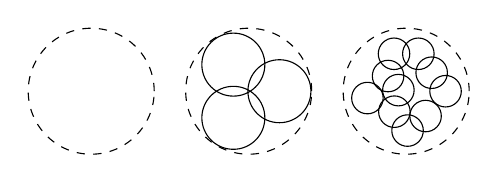
\begin{tikzpicture}
    % spherical proton
    \draw[dashed, xshift=-2cm] (0,0) circle (.8cm);
    % three partons
    \draw[dashed] (0,0) circle (.8cm);
    \foreach \theta in {0, 120, 240}{
      \draw ({\theta}:.39) circle (.4cm);
    }
    % ten partons
    \draw[dashed, xshift=2cm] (0,0) circle (.8cm);
    \foreach \theta/\radius in {
      36/0.4, 72/0.5, 108/0.5, 140/0.3, 172/0.1,
      190/0.5, 240/0.3, 272/0.5, 308/0.4, 360/0.5
    }{
      \draw[xshift=2cm] ({\theta}:\radius) circle (.2cm);
    }
  \end{tikzpicture}
  \caption{\label{proton_shapes} Schematic of plausible proton shapes.
  The sketch on the left shows a spherically symmetric proton (dashed line), while the middle and right illustrations depict a fluctuating proton with three and ten partons respectively (solid lines).
  }
\end{figure}

\section{Parameter estimation}

\subsection{Computer experiment design}

\subsection{Gaussian process emulators}

\subsection{Bayesian calibration}

Aliquam porttitor massa risus, hendrerit dignissim purus placerat vel. Suspendisse dui ante, porttitor pretium lorem et, placerat posuere mi. Donec lacinia nisl leo, ac luctus libero tincidunt non. Donec pretium ultricies felis vitae tempus. Duis pulvinar nisi justo, sit amet finibus orci volutpat non. Proin fermentum a magna id rhoncus. Vestibulum posuere, ipsum vel dignissim laoreet, arcu nibh venenatis neque, et aliquet dui dui a ipsum. Praesent sagittis condimentum neque, sed aliquam odio volutpat nec. Aenean consequat ante eget mauris lacinia, sed ultrices est dapibus. Morbi fermentum malesuada turpis, ac placerat est bibendum tincidunt. Nullam leo ipsum, sodales sit amet viverra non, iaculis vel nisl. Vestibulum purus ipsum, egestas ut bibendum sed, congue quis purus. Curabitur iaculis tortor nisl, nec venenatis tortor placerat a. Fusce feugiat nisl vitae porta porta. Praesent non arcu leo. Sed gravida eget neque in auctor.


Sed ac ullamcorper ipsum. Sed quis eleifend mauris. Phasellus quis massa neque. Proin nec lectus quis ante aliquam tincidunt ut sit amet eros. Nullam et odio eu elit aliquam molestie quis ut arcu. Aliquam gravida enim non tortor bibendum, at semper tellus egestas. In libero lectus, convallis in suscipit nec, bibendum eu felis. Vestibulum ante ipsum primis in faucibus orci luctus et ultrices posuere cubilia Curae; Vivamus quis lectus neque. Sed ac placerat justo. Nullam ultricies vulputate ligula, vel porta mauris scelerisque et. Sed hendrerit blandit semper. Sed vel bibendum elit, eu posuere elit. Phasellus nunc massa, tincidunt ac tempus quis, blandit quis erat. 


\section{Results}

\subsection{Initial condition properties}

\subsection{QGP medium properties}

Aliquam porttitor massa risus, hendrerit dignissim purus placerat vel. Suspendisse dui ante, porttitor pretium lorem et, placerat posuere mi. Donec lacinia nisl leo, ac luctus libero tincidunt non. Donec pretium ultricies felis vitae tempus. Duis pulvinar nisi justo, sit amet finibus orci volutpat non. Proin fermentum a magna id rhoncus. Vestibulum posuere, ipsum vel dignissim laoreet, arcu nibh venenatis neque, et aliquet dui dui a ipsum. Praesent sagittis condimentum neque, sed aliquam odio volutpat nec. Aenean consequat ante eget mauris lacinia, sed ultrices est dapibus. Morbi fermentum malesuada turpis, ac placerat est bibendum tincidunt. Nullam leo ipsum, sodales sit amet viverra non, iaculis vel nisl. Vestibulum purus ipsum, egestas ut bibendum sed, congue quis purus. Curabitur iaculis tortor nisl, nec venenatis tortor placerat a. Fusce feugiat nisl vitae porta porta. Praesent non arcu leo. Sed gravida eget neque in auctor.

Sed ac ullamcorper ipsum. Sed quis eleifend mauris. Phasellus quis massa neque. Proin nec lectus quis ante aliquam tincidunt ut sit amet eros. Nullam et odio eu elit aliquam molestie quis ut arcu. Aliquam gravida enim non tortor bibendum, at semper tellus egestas. In libero lectus, convallis in suscipit nec, bibendum eu felis. Vestibulum ante ipsum primis in faucibus orci luctus et ultrices posuere cubilia Curae; Vivamus quis lectus neque. Sed ac placerat justo. Nullam ultricies vulputate ligula, vel porta mauris scelerisque et. Sed hendrerit blandit semper. Sed vel bibendum elit, eu posuere elit. Phasellus nunc massa, tincidunt ac tempus quis, blandit quis erat. 

\section{Summary and conclusions}

Aliquam porttitor massa risus, hendrerit dignissim purus placerat vel. Suspendisse dui ante, porttitor pretium lorem et, placerat posuere mi. Donec lacinia nisl leo, ac luctus libero tincidunt non. Donec pretium ultricies felis vitae tempus. Duis pulvinar nisi justo, sit amet finibus orci volutpat non. Proin fermentum a magna id rhoncus. Vestibulum posuere, ipsum vel dignissim laoreet, arcu nibh venenatis neque, et aliquet dui dui a ipsum. Praesent sagittis condimentum neque, sed aliquam odio volutpat nec. Aenean consequat ante eget mauris lacinia, sed ultrices est dapibus. Morbi fermentum malesuada turpis, ac placerat est bibendum tincidunt. Nullam leo ipsum, sodales sit amet viverra non, iaculis vel nisl. Vestibulum purus ipsum, egestas ut bibendum sed, congue quis purus. Curabitur iaculis tortor nisl, nec venenatis tortor placerat a. Fusce feugiat nisl vitae porta porta. Praesent non arcu leo. Sed gravida eget neque in auctor.

Sed ac ullamcorper ipsum. Sed quis eleifend mauris. Phasellus quis massa neque. Proin nec lectus quis ante aliquam tincidunt ut sit amet eros. Nullam et odio eu elit aliquam molestie quis ut arcu. Aliquam gravida enim non tortor bibendum, at semper tellus egestas. In libero lectus, convallis in suscipit nec, bibendum eu felis. Vestibulum ante ipsum primis in faucibus orci luctus et ultrices posuere cubilia Curae; Vivamus quis lectus neque. Sed ac placerat justo. Nullam ultricies vulputate ligula, vel porta mauris scelerisque et. Sed hendrerit blandit semper. Sed vel bibendum elit, eu posuere elit. Phasellus nunc massa, tincidunt ac tempus quis, blandit quis erat. 

\begin{acknowledgments}
  The authors thank ...
\end{acknowledgments}

\bibliography{trento-partons}

\end{document}
